\frame{
\frametitle{Cómputo de alto rendimiento (HPC)}
% https://www.usgs.gov/core-science-systems/sas/arc/about/what-high-performance-computing

\begin{itemize}
\item El HPC se refiere a sistemas informáticos con una potencia computacional extremadamente alta que son capaces de resolver problemas enormemente complejos y exigentes, como son aquellos relacionados a ciencia, ingeniería o negocios.
\item Algunas barreras computacionales típicas:
    \begin{itemize}
        \item Tiempo: el procesamiento en los sistemas locales es demasiado lento o no es factible.
        \item Capacidad de la CPU: solo se puede ejecutar un modelo a la vez. Desarrollar, implementar y difundir técnicas y herramientas de vanguardia para que los modelos se apliquen de manera más eficaz a la toma de decisiones actual.
    \end{itemize}
\end{itemize}


}

\frame{
\frametitle{Cómputo paralelo}
%https://hpc.llnl.gov/training/tutorials/introduction-parallel-computing-tutorial
En el sentido más simple, el cómputo paralela es el uso simultáneo de múltiples recursos de computación para resolver un problema computacional
\begin{itemize}
\item Un problema se divide en partes discretas que se pueden resolver al mismo tiempo.
\item Cada parte se desglosa además en una serie de instrucciones.
\item Las instrucciones de cada parte se ejecutan simultáneamente en diferentes procesadores
\item Se emplea un mecanismo de control / coordinación general
\end{itemize}
\begin{block}{¿Porqué utilizar cómputo paralelo?}
El mundo real es enormemente complejo, ya que muchos eventos complejos e interrelacionados están sucediendo al mismo tiempo, pero dentro de una secuencia temporal. En comparación con la computación en serie (Von Neumann), el cómputo paralelo es mucho más adecuado para modelar, simular y comprender fenómenos complejos del mundo real.
\end{block}
}


\frame{
\frametitle{Paralelismo Espacial}
\begin{columns}
  \column {0.5\textwidth}
  \begin{itemize}
\item Normalmente, las instrucciones de los programas escritos en cualquier lenguaje de alto nivel se ejecutan en serie, es decir, una instrucción tras otra.
\item Sin embargo, las máquinas modernas tienen varios núcleos (cores), lo cual permite ejecutar los problemas para que puedan ejecutarse simultáneamente en paralelo y obtener una gran aceleración.
\item Lo anterior esta limitado por el número de núcleos del procesador.
  \end{itemize}
    \column {0.5\textwidth}  
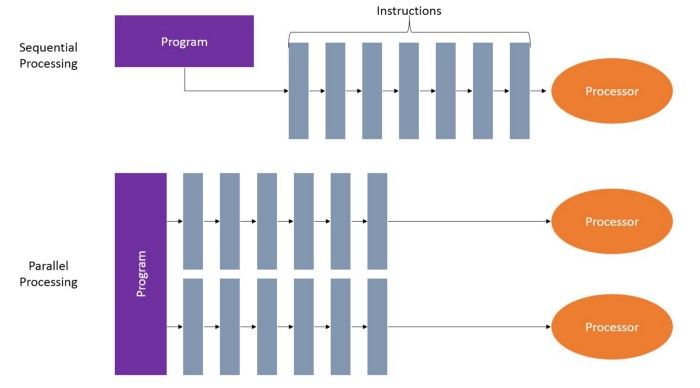
\includegraphics[width=0.9\textwidth]{Figs/SecuentialvsParallelComputing}  
  \end{columns}
}


\frame{
\frametitle{Paralelismo Temporal (Pipeline)}
\begin{columns}
  \column {0.5\textwidth}
  \begin{itemize}
\item Cuatro individuos (A,B,C,D) requieren llevar a cabo una serie de tareas (lavar, secar, doblar y acomodar)
\item Cada proceso toma 30 minutos.
\item En una lavandería secuencial, cada individuo debe esperar a que termine el anterior y así consecutivamente (tiempo total: 8 horas).
\item En una lavanderia en Pipeline, los individuos empezarían sus tareas uno detrás del otro, sin esperar a que el anterior las cuatro tareas (tiempo total: 3 horas y 30 minutos). 
%Este proceso seguiria hasta que todos realicen sus tareas, y el tiempo para que esto suceda ahora sería de 3 horas y 30 minutos. 
  \end{itemize}
    \column {0.5\textwidth}  
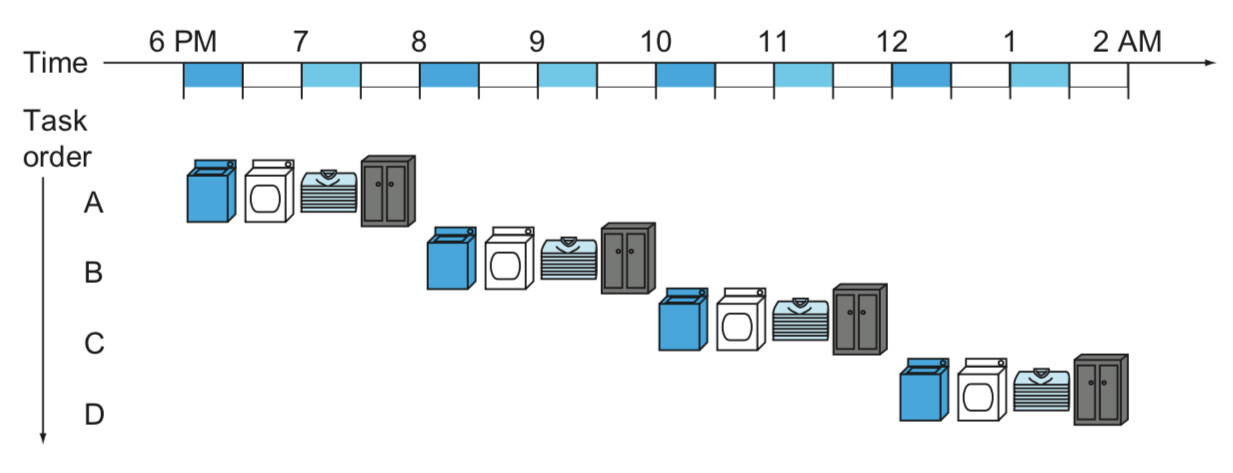
\includegraphics[width=0.9\textwidth]{Figs/computer-architecture-4-5-1}\\
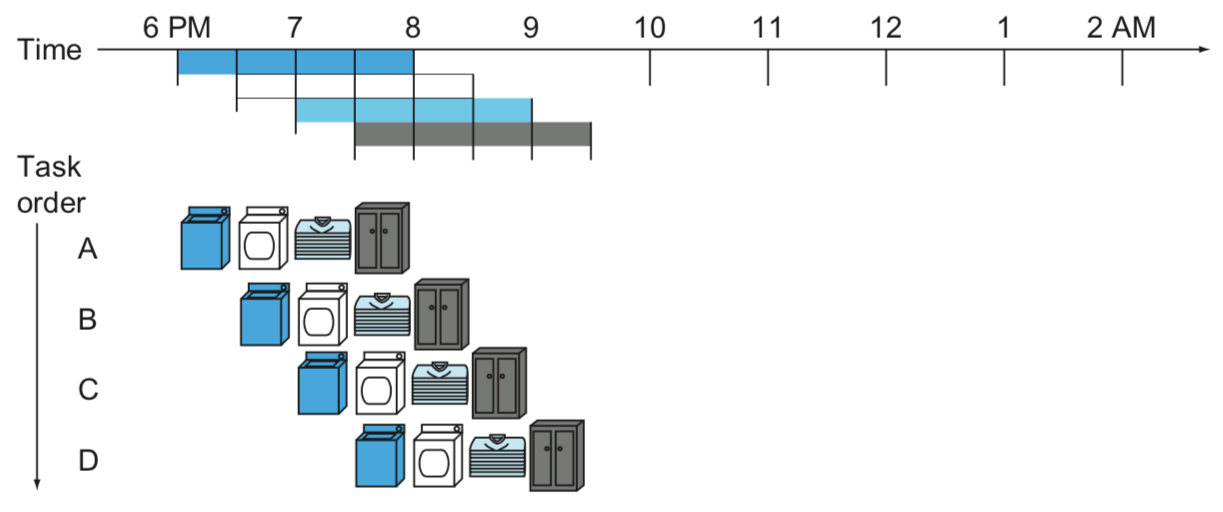
\includegraphics[width=0.9\textwidth]{Figs/computer-architecture-4-5-2}   
  \end{columns}
}


